\chapter{Background and Related Work}
In this chapter, the reader is introduced to physics simulations and the differences between real-time and non-real-time simulations along with important terms, workings, important and relevant aspects of physics simulations. Along with an introduction to physics simulations, the following points will also be discussed:
\begin{itemize}
	\item Scalable Non-Real-Time physics
	\item Physics in online gaming
	\item Graph-partitioning
	\item Distributed virtual environments
	\item Distributed real-time physics
	\item Cloud computing
	\item Scientific and Engineering simulations
	\item Containerisation of game engines
	\item Streamed gaming
\end{itemize}

\section{Real-time Physics Engines Overview}
%We introduce the reader to the topic of physics simulations and we compare real-time with non-real-time physics simulations. We define terms, workings, important and relevant aspects, e.g. body types, uses in games and simulations, typical scales and performance of real-time simulations and performance budget in real-time applications.

Real-time physics simulations (physics engines) are responsible for simulating the physical behaviour of objects and are based around Newtonian mechanics. The motion of the system is calculated given the forces acting on the system, this is known as the forward dynamics problem \cite{Boeing2007}.

The main three aspects of the functionality of a physics engine are the following:
\begin{itemize}
	\item Integration: Moving objects according to a set of physical rules and values i.e. velocity, drag, friction
	\item Collision Detection: Checking for collisions between two or more objects
	\item Collision Response: The reaction to collisions between objects
\end{itemize}

The term `object' is used here to describe any physical entity. Objects can be any entity that physically interacts, for example, a barrel, a bullet, a fire particle, a jointed robot arm, the wheel of a vehicle, a mountain etc. The terms `world' or `scene' are often used to describe the physical system.

The numerical integrator used to update the positions of objects in the system, uses a discrete time value for each step, this is known as the time step. Each step simulates a set period of time. The shorter the time period simulated, the more physically accurate the simulation will be, however, each simulation step must take less time to execute than the time it is intending to simulate, otherwise the simulation would be unable to run in real-time. It is common for the time step to be a fixed value, though physics engines can support variable time steps.

\subsection{Linear Motion}
Linear motion will first be discussed and the following variables are used:
\begin{itemize}
	\item $F$ - Force
	\item $m$ - Mass
	\item $a$ - Acceleration
	\item $v$ - Velocity
	\item $s$ - Displacement
	\item $n$ - Current time step
	\item $n+1$ - Next time step
\end{itemize}

Acceleration is calculated from the sum of the forces acting on the body and with the use of the mass of the objects and Newton's Second Law:

\begin{equation}
F=ma
\end{equation}

The simplest numerical integrator is explicit Euler (or sometimes referred to simply as Euler) integration:

\begin{equation}
\begin{split}
	v_{n+1}=v_n+a_{n+1}{\Delta}t\\
	s_{n+1}=s_n+v_{n}{\Delta}t
\end{split}
\end{equation}

However, this is not often used by physics engines as it can lead to instability unless short time steps are used.

A Symplectic Euler (Semi-Implicit Euler) Integrator is often used in physics engines. Symplectic Euler is similar to explicit Euler, except that the updated velocity is used before calculating the new position:

\begin{equation}
\begin{split}
	v_{n+1}=v_n+a_n{\Delta}t\\
	a_{n+1}=a_n+v_{n+1}{\Delta}t
\end{split}
\end{equation}

Symplectic Euler is faster to compute and remains accurate over many iterations and is stable when longer time steps are used.

\subsection{Angular Motion}
In addition to solving linear motion, physics engines also solve angular motion. Angular motion will now be discussed and the following variables are used:
\begin{itemize}
	\item $T$ - Torque
	\item $I$ - Inertia Matrix or Inertia Tensor
	\item $\alpha$ - Angular acceleration
	\item $\omega$ - Angular velocity
	\item $\theta$ - Orientation
	\item $n$ - Current time step
	\item $n+1$ - Next time step
\end{itemize}

Orientation of objects are represented using Quaternions. Torque is calculated using the following equation:

\begin{equation}
T=I\alpha
\end{equation}

This equation is the rotational equivalent of $F=ma$.
%Inertia
Angular velocity $\omega$ can be integrated relative to angular acceleration $\alpha$ using the following equation:

\begin{equation}
\omega_{n+1}=\omega_n+\alpha_n\Delta t
\end{equation}

Orientation $\theta$ can then be calculated using $\omega$ and the following equation:

\begin{equation}
\theta_{n+1}=\theta_n+\theta_n\omega_n\frac{\Delta t}{2}
\end{equation}

This equation is a fast approximation of orientation.

\subsection{Integration comparison with non-real-time simulations}
The equations used in real-time physics engines use iterative processes and approximate a continuous process with discrete steps. As a result, errors due to inaccuracies in the discreteness accumulate over time due to the iterative nature of the integrators. Different real-time physics engines will often give different results for the same simulation, despite identical starting parameters \cite{Boeing2007}.

\subsection{Collision Detection}\label{collision_detection}
Objects are represented by geometry colliders. Collision detection works by detecting overlaps between geometry representations.
Typically objects have simple colliders, such as boxes, capsules, cylinders and spheres. More complex colliders are often supported, such as convex and concave hulls. Colliders can either be static or dynamic.

Optimisations for collision detection are used to avoid comparing every possible pair of objects. Phases of collision detection are used, known and the broadphase and the narrowphase.
%TODO: Give examples of these



%Collision detection
%Collision response
%Constraints
%Body describes any non-point-like physical entity

%Main physics loop (what goes on within a simulation step)
%Explanation of rigid bodies, actors, shapes, constraints
%Explanation of simulation and query shapes
%Explanation of trigger volumes
%Explanation of kinetic vs kinematic
%Explanation of sleeping

%It is possible for the main application to update more often than the simulation frequency
%It is also possible that the main application update is unable to be executed at the same frequency as the physics simulation frequency. Options are running the simulation at a bigger time-step or simulate multiple, smaller sub-steps. Trade-off between keeping consistent behaviour and performance.
%Diagrams for above
%Well of despair example and diagram
%Solutions to well of despair: 
%Decouple physics from application update with use of sync and async scene, can make player interaction more difficult
%allow time dropping
%variable time-stepping
%simplifying the physics scene

%PhysX runs on a separate thread by default
%It is not possible to read/write directly to the scene during simulation, scene is buffered so changes can be made and will only affect the next simulation step. 
%Image of time-slots
%Event callbacks for collisions/triggers

\subsection{Collision Response}

%\subsection{Constraints}

\subsection{Performance of Real-Time Physics Engines}
In this section the performance of real-time physics engines will be discussed. Examples of different scenarios under different performance conditions will be used and discussed using time-sequence diagrams.

Physics engines are kept as separate as possible from the rendering loop and other logic in the main loop. Fig. \ref{GoodPerf} shows a time sequence diagram of a game loop with good performance. The target physics time step is 16ms. Every 16ms that is passed, a physics update is triggered, simulating 16ms of the simulation. Multiple update loops can be completed between physics steps being performed.

\begin{figure}
	\centering
	\input{Figs/GoodPerfNoVSync.pdf_tex}
	\caption{Time sequence diagram of good performance.}
	\label{GoodPerf}
\end{figure}

Fig. \ref{SubStep} shows a time sequence diagram of sub-stepping. If an update loop takes longer than the target time-step (in this case 16ms), multiple physics steps will need to be performed to update the simulation to the present time. This is known as sub-stepping. Sub-stepping is supported by PhysX. Longer update times may occur in many situations, such as a read from the hard-drive, a background process performed by the OS or particularly expensive game logic or AI task.

\begin{figure}
	\centering
	\input{Figs/SubStepping.pdf_tex}
	\caption{Time sequence diagram of sub-stepping.}
	\label{SubStep}
\end{figure}

Fig. \ref{ExpensivePhysics} shows a time sequence diagram of a scenario in which the simulation is expensive to update. This could be the result of a large number of objects being simulated or complex collision detection. As a result of the expensive physics update the render frame rate is reduced to 60Hz, despite the main update only taking $~3ms$.
%TODO: Expand this?

\begin{figure}
	\centering
	\input{Figs/ExpensivePhysics.pdf_tex}
	\caption{Time sequence diagram of expensive physics.}
	\label{ExpensivePhysics}
\end{figure}

%Fig. \ref{WellOfDespair} shows a time sequence diagram of a scenario in which a long update frame has occurred. The main update has taken long enough that two sub-steps must be simulated, as each sub-step takes $~9ms$, it will take $~18ms$ to simulate. As a result, the time step also misses the target of $16ms$, 
%
%\begin{figure}
%	\centering
%	\input{Figs/WellOfDespair.pdf_tex}
%	\caption{The well of despair.}
%	\label{WellOfDespair}
%\end{figure}

\section{Scalable Non-Real Time Physics}
Scalable Non-Real Time Physics include fluid simulations, meteorological simulations and accurate physical simulations e.g. robotics, wheeled and tracked vehicle dynamics and mechatronics. An example of a Scalable Non-Real Time Physics is Project Chrono \cite{Chrono}. Non-real time physics simulation work very differently from real-time, accuracy is highly favoured as opposed to the fast, plausible simulations in real-time physics. In addition high latency (10s of ms) is a small issue relative to large time-steps used in such simulations.

\section{Online Gaming}
In this section an overview of online gaming challenges and system architectures will be discussed. 

The main challenges facing online gaming are consistency, latency, fault-tolerance, fairness, cheating, and scalability.

\subsection{Consistency}
Consistency, as online games are distributed (either between clients and a server, peers or multiple servers), inconsistent states can occur. Multiple peer/servers execute updates in parallel, however if these are executed out of order, such as due to messages being received out of order, inconsistent states can arise.  Different aspects of game state require different levels consistency and games often employ consistency resolution instead of inconsistency prevention \cite{P2PSurvey}.

%Strong Consistency
%Weak Consistency
%2 of 3, availability, network partitioning, consistency
%An Enhanced Dead Reckoning Model for Physics-Aware Multiplayer Computer Games
%Peer-to-Peer Architectures for Massively Multiplayer Online Games: A Survey
%TODO: Talk about consistency in Proposed Solution

\subsection{Latency}
Latency can significantly affect the quality of experience of a game and can impact both a player's performance in a game \cite{EffectsofLossandLatency, claypool2010latency} and subjective perception of the game \cite{dick2005analysis}. However, this depends heavily on the game genre and actions taken by the player \cite{LatencyandPlayerActions, claypool2010latency}. Fig. \ref{fig_LatencyCompensation} shows an example of the effects of latency on a networked game. Where the target appears to the player and hitboxes on the server used to detect a player's shot are significantly different.

% Latency and scalability: a survey of issues and techniques for supporting networked games
% Synchronization Technique - Lock-step
% Optimistic Technique
%TODO: Talk about latency compensation in Proposed Solution

\begin{figure}
	\centering
	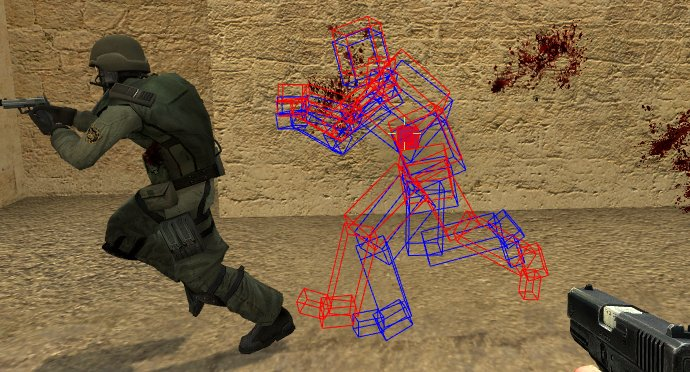
\includegraphics[width=\textwidth]{Figs/LagCompensation.jpg}
	\caption{ A screenshot taken when 200ms of latency was present on a client. The red hitboxes show the target position on the client (100ms + interpolated period). While the user command was travelling to the server, the target continued to move to the left. When the user command arrived at the server, the server reverted the target position (blue hitboxes) using the estimated time of the command execution. The server calculates whether or not the hist was successful and sends a confirmation message to the client \cite{Source}.}
	\label{fig_LatencyCompensation}
\end{figure}

\subsection{Fault-tolerance}
Fault-tolerance is a challenge for online gaming and can result from failures or unscheduled disconnections of server or peers which can lead to the loss of game state \cite{P2PSurvey}.

\subsection{Fairness}
Fairness is the degree of difference among all players’ gaming environments, i.e. players should be treated equally and no game advantage/disadvantage should be given to players due to factors like latency \cite{P2PSurvey}.

%MANAGING LATENCY AND FAIRNESS IN NETWORKED GAMES 

\subsection{Cheating}
Cheating is when players maliciously gain an unfair advantage in a game. Cheating reduces the quality of experience for non-cheating players and is a main concern in the design of game architecture \cite{P2PSurvey}. 

\subsection{Scalability}
Scalability in online games is measured in terms of players that can be supported \cite{turchini2015scalability}. An online gaming system's ability to scale depends upon the architecture employed. The different architectures than can be used will now be discussed.

%This screenshot was taken on a listen server with 200 milliseconds of lag (using net_fakelag), right after the server confirmed the hit. The red hitbox shows the target position on the client where it was 100ms + interp period ago. Since then, the target continued to move to the left while the user command was travelling to the server. After the user command arrived, the server restored the target position (blue hitbox) based on the estimated command execution time. The server traces the shot and confirms the hit (the client sees blood effects).

%Client and server hitboxes don't exactly match because of small precision errors in time measurement. Even a small difference of a few milliseconds can cause an error of several inches for fast-moving objects. Multiplayer hit detection is not pixel perfect and has known precision limitations based on the tickrate and the speed of moving objects. 

\subsection{Architectures}
Online game architectures fall into the following main categories client-server, peer-to-peer, hybrid peer-to-peer and distributed server (also referred to as multiserver). Each type has advantages and disadvantages and suitability depends on a number of factors, including number of players and whether or not the game is short-session-based or persistent.
%We discuss the wider topic of online gaming (client-hosted, P2P, server), challenges of latency, security/cheating and computational limits. Also some details of online gaming servers are discussed, specifically, typical server frame-times and network tick updates.

\subsubsection{Client-Server}
Client-Server architecture is a type of architecture in which the game is executed and game state is managed entirely by the server. Clients connect to the server and receive the necessary information about the game world. All messages and interactions are sent through the game server and the server is responsible for disseminating messages to the appropriate clients. The main challenge with this approach is scalability, as a single server can only support a limited number of players. This is normally solved with the addition of more servers, i.e. switching to a distributed server architecture. As all communication goes through the server, clients do not directly communicate with each other, meaning latency can be increased for interactions with other players.
As there is only one central version of the game state, consistency resolution is simplified to solving inconsistencies between server and client and the server treated as the correct master copy. In addition, fault-tolerance is simplified to keeping a single backup of the central server's sate, although this adds more complexity and cost, and can reduce scalability. Client-Server architectures are less prone to cheating than peer-to-peer based architectures, as the game provider has complete control over the game state \cite{P2PSurvey}.

\begin{figure}
	\centering
	\input{Figs/ServerHosted.pdf_tex}
	\caption{Server hosted networked game.}
\end{figure}

%\subsection{Client-Hosted}
%
%\begin{figure}
%	\centering
%	\input{Figs/ClientHosted.pdf_tex}
%	\caption{Client hosted networked game.}
%\end{figure}

\subsubsection{Peer-to-Peer}
Peer-to-Peer, often referred to as`P2P', is a type of architecture in which the game is executed and game state is managed entirely by the peers, although peers are often only responsible for a subset of the game state, such as the entities they are currently interacting with. A peer-to-peer architecture is shown in Fig. \ref{fig_P2P}. Peers are all responsible for message forwarding to each other. In other words, peers act as bother server and client. Peer-to-Peer reduces the cost for the game provider of maintaining expensive servers and can reduce latency between players, as communication is performed directly between peers, rather than communicating through a server. In addition, it provides scalability in terms of compute power, as the more peers that join, the more resources available to the system. However, as more peers join, the greater the communication overhead is between peers. In addition, peer-to-peer is prone to the problems of fault-tolerance, data consistency and cheating by players. A peer is more likely to fail or experience unscheduled disconnection than a dedicated server. As each peer is responsible for the game state, it is possible for communication errors to occur, resulting in two peers with different game states or a peer maliciously altering the game state or the messages being sent to other peers in order to cheat. The fault-tolerance requirements of peer-to-peer can be reduced in short-session-based games, making these architectures better suited to those games \cite{P2PSurvey}. Peer-to-Peer architectures have received much research attention in previous years, with many solutions that attempt to address the problems above, through the use of techniques discussed in \cite{P2PSurvey}.

%VoroGame, work is distributed amongst clients.
%VoroGame uses Voronoi spatial partitioning to assign a region to a peer and an overlay based on a distributed hash table for data distribution.

\begin{figure}
	\centering
	\input{Figs/PeerToPeer.pdf_tex}
	\caption{Peer-to-peer hosted networked game.}
	\label{fig_P2P}
\end{figure}

\subsubsection{Hybrid Peer-to-Peer}
Hybrid Peer-to-Peer architectures are a combination of client-server and peer-to-peer architectures. The peer-to-peer part of the system can be responsible for different aspects of the system, including Cooperative Message Dissemination, State Distribution, Basic Server Control and distributing software updates. \cite{P2PSurvey}. Hybrid Peer-to-Peer enable trade-offs between consistency control and scalability are enabled, depending on how the system is divided between server and peer-to-peer.
%These can be broadly classified into two types: Homogeneous, in which all nodes have similar responsibilities and Heterogeneous, in which some peers be

\subsubsection{Distributed server}
% TODO: More references for this
Distributed server or Multi-Server architectures use multiple servers and the computational workload is divided between the servers. This can be achieved in one of two ways, either through `shards' or through division of the game world. 

In the `shards' method, complete and separate instances of the game world exist, each maintained by one serve. Each server is responsible for a different set of clients. The game can be scaled through the introduction of more servers, supporting more clients. However, as each instance of the game world is separate, there can be no interaction in the game world between players on different shards \cite{P2PSurvey}.

In the game world division method, there is a single instance of the game world and the workload is distributed either through each server being responsible for a region or a set of players. Division methods are discussed further in \ref{distrubted_virtual_env}. 
a single server can be overloaded if the workload is too high, for example, by a large number of players in a region being managed by a single server. Dynamic load-balancing schemes can be employed to improve distribution between servers. The disadvantage of this approach is the need for complex hand-offs when players migrate or interact between servers and can lead to consistency problems between servers as latency will always exist between servers \cite{P2PSurvey}.

The distributed server approach enables scalability as more servers can be utilised, allowing support for more players. However, depending on workload distribution, more problems are introduced. Fault-tolerance is potentially higher than a single server solution, even if no backup system is employed, as only players connected to the failing server will be affected \cite{P2PSurvey}.

%TODO: Mention cost? Persistent games?

\subsection{Update Rate and Network Tick Rate} \label{update-rate-test-values}

Two important aspects of online video game servers are the update rate and network tick rate, which will now both be defined. Update rate is the rate at which the server updates the game state, such as game logic updates and AI. Network tick rate is the rate at which the server communicates the game state to clients and clients communicate interactions with the server, such as movement input for a player character \cite{pisan2004challenges}. The two rates can be independent of each other and the network tick rate can be lower than the server update rate, reducing the network requirements through less frequent communication between server and client.

In many cases it is not possible for a server to communicate the entire game state to the each client due to bandwidth constraints. Instead, techniques are used to prioritise and filter the information that is most relevant to each client, in order to reduce the data that needs to be communicated with clients \cite{pisan2004challenges}. These techniques are known as Interest Management and discussed further in \ref{InterestManagement}.

The rates chosen for network tick rates depend on a variety of factors, including the required level of accuracy and bandwidth restrictions. Higher tick rates enable higher accuracy, but at the cost of more bandwidth being required. Different genres of games have different accuracy demands. For example, in first-person-shooters (FPS), higher tick rates result in a higher mean shooting accuracy for players \cite{lee2015evaluation}. Whereas, genres like real-time-strategy (RTS) games have more relaxed accuracy requirements. In the RTS Age of Empires, latency only became noticeable if it exceeded $500ms$, meaning network tick rates can be very low without being noticeable to the player \cite{pisan2004challenges}. Tick rates of popular network games range from 128Hz for CS:GO to 20Hz for Minecraft \cite{metzger2016comprehensive}.

%TODO: Mention delta-update techniques, advantages and problems created

%Dale's work starts here
%The ideal update rate depends on a number of factors such as the complexity of the simulation, the required level of accuracy, the number of network peers involved, and availability of bandwidth. Some simulations with large environments may need to send and receive large network packets. If a competitive video game requires fast reaction times and tight synchronisation between a client and a server, it may use a higher update rate - for example, competitive sessions of \textit{Counter-Strike} may use an update rate of 60Hz or more. In contrast, a game such as \textit{Minecraft} that does not require this level of responsiveness but does offer large environments could use a lower update rate of 20Hz to conserve bandwidth and reduce processing overheads \cite{lee2015evaluation}.

%For our tests, we chose a variety of popular update rates found in recent triple-A video games: 10Hz, 30Hz, and 60Hz. 10Hz was used by \textit{Battlefield 4} at launch, and later changed to 30Hz after a software update in response to player feedback regarding poor online experience, and so this represents a low update rate. 30Hz is used by many console games or games with large environments, and could be considered an average update rate. 60Hz is used by games that require fast response times (i.e. competitive first-person shooters) and so it represents a high update rate.

%To achieve these update rates, a ``frame-time'' parameter is present in the simulation, which controls how long a complete frame (physics time step and network update combined) should take in milliseconds by delaying execution appropriately.
%Dale's work ends here


\section{Physics in Online Gaming}
%(and the lack of, due to the challenges faced). Mostly limited to dead-reckoning
%https://books.google.co.uk/books?hl=en&lr=&id=ujfOBQAAQBAJ&oi=fnd&pg=PA307&dq=Physics+networked+games&ots=OC5YWxmd25&sig=vcxatd9Wl0_SdxCAUZvmP6BWl7I&redir_esc=y#v=onepage&q=Physics%20networked%20games&f=false

%Predictive schemes that run locally

\section{Graph-Partitioning}
%When it comes to spatially-partitioning a simulation, the problem is essentially a graph partitioning problem, where objects are nodes and if there’s a possible interaction, an edge exists. Useful for terms, comparisons with and future work on load-balancing will heavily involve this.

\section{Distributed Virtual Environments} \label{distrubted_virtual_env}
%We look at existing ways of distributing game worlds and previous work carried out on these approaches. These fall into two categories, migratory (approach used by AP) and non-migratory. The studies found non-migratory to be the better solution when focusing on player-player interaction and we will discuss why migratory is the better solution for physics body-physics body interaction. Important concepts such as interest management are introduced to the reader.

Although there has been research utilising multiple servers to distribute the task of solving physics based problems (e.g., \cite{mashayekhi2018automatically}), to the best of our knowledge there is no literature describing real-time interactive physics exploiting the addition of servers to gain scalability. The closest work to our research is that carried out to seek scalability in terms of player numbers in online gaming in the field of Distributed Virtual Environments (DVEs). 

There are primarily two ways in which server-side resources can provide scalability in online gaming (e.g., DVEs): (1) Migratory; (2) Non-migratory. In migratory approaches, a server will assume responsibility for handling in-simulation objects within a region. When objects traverse region boundaries into a region that is the responsibility of another server, they will be handed over to the other server. In a non-migratory approach, in-simulation objects are allocated to the responsibility of a particular server at instantiation time and stay with that server until they are deleted.

The benefit of a migratory approach is that tightly coupled objects (interacting frequently) can be co-located on the same server, reducing interaction latencies. However, the act of moving such objects may be costly in terms of time required to resolve the hosting requirements of an object. The benefit of a non-migratory approach is that servers are rarely exhausted but network traffic will result in higher latencies that will inhibit the fidelity of interaction between objects.

Migratory and non-migratory approaches are now described in greater detail.

In the migratory approach, a single game world exists, but is divided into geographical regions. Each region is maintained by a separate server (e.g. \cite{AnOverlappingArchitecture, ScalabilityIssues, LoadBalancingForDistributedVR, ALoadBalancingAlgorithm, SpatialOS}). The main drawback of this approach is the complexity of handling interactions between objects in different regions/servers while maintaining consistency \cite{P2PForMMOs}. A technique to minimise these issues is to use overlapping regions between spatial partitions. Servers share state information about objects in the overlapping region (examples include 'zoning' as described in \cite{AnOverlappingArchitecture} or 'sub-regions' as described in \cite{ScalabilityIssues}). Examples of games using this technology include \cite{Vanishin30:online} and \cite{WorldsAd48:online}, which use the SpatialOS platform \cite{SpatialOS}. %However, the techniques used by SpatialOS are not described in any literature. Their demonstration video exhibits unnatural object "jitter", which is possibly a result of network latency. 
 
In the non-migratory approach, the game world is not divided into geographical regions and players are split between servers in one of two ways: (1) Several instances of the game world run with complete independence from one another (known as shards e.g.\cite{WOW}) and players have no interaction across shards \cite{P2PForMMOs}; (2) Players are distributed amongst servers by some other non-geographical method and interactions with players on other servers requiring servers to share messages \cite{LoadBalancingforMMOs}.

Although shards allow a degree of scalability in the number of players, it is not suitable for use in scaling real-time physics simulations as all entities within a real-time physics simulation, in the same geographical region, may interact with each other.

In the case of architectures not using shards, Interest Management is required to prevent message passing growing polynomially as players increase (e.g. \cite{Bezerra2008} and \cite{LoadBalancingforMMOs}).
\cite{Bezerra2008} proposes the A3 algorithm, an interest management technique for distributed simulations aiming to significantly reduce the necessary bandwidth required between servers. A3 uses a combination of a circular area of interest and field of view combined with a relevance gradient. \cite{LoadBalancingforMMOs} proposes a Behavioural Interest Management Technique that allocates resources based on player interactions. Auras (an area of interest/influence) are used to determine player message exchanges, reducing message passing while promoting player number scalability.

Despite DVE being a popular area of research, the literature is restricted to modelling player interaction across servers and balancing their support on different servers. Clearly, the interaction patterns of players are significantly less demanding in terms of timeliness than that of interacting physical objects.


% Some introduction to interest management?
\subsection{Interest Management}\label{InterestManagement}
The technique presented in this paper, Aura Projection, makes use of the aura concept from Interest Management. Interest Management is a term used to describe any method of restricting message dissemination between objects within a virtual space, with the aim of reducing the network overhead when large numbers of participants or players are connected to a virtual world \cite{Morgan2005}.

Interest Management can be broadly classified into two categories: Regions and Auras \cite{Morgan2005, storey2004determining}.
\subsubsection{Regions}
``In the region based approach the virtual world is commonly, but not always, divided into well defined uniform sized regions that are static in nature (i.e. their boundaries are defined at virtual world creation time)."\cite{storey2004determining}
\subsubsection{Auras}
``In the aura based approach each object is associated to an aura that defines an area of the virtual world over which an object may exert influence. Ideally, an object may potentially communicate their actions to only objects that fall within their influence."\cite{storey2004determining}\\

Interest Management is relevant to our work as it enables the minimisation of network overhead in distributed virtual environments. It is important to note that objects within a virtual space are only affected by other objects in their region and neighbouring regions or objects within their area of influence. Aura Projection uses the concept of auras to minimise message passing between servers while still allowing time-space consistency to be maintained.

In addition to reducing the network traffic between servers, interest management can also be utilised to reduce the required network traffic between client and servers. In terms of physics being simulated on server(s), clients will be most concerned with objects within close proximity to them and less concerned with objects beyond the range in which can be physically interacted with. In addition, clients will be more concerned with objects in their field of view than objects that can't currently be seen. An example of an interest management technique using distance and field of view is \cite{Bezerra2008}. \cite{Bezerra2008} proposes the A3 algorithm, an interest management technique for distributed simulations aiming to significantly reduce the necessary bandwidth required in a distributed game server. A3 uses a combination of a circular area of interest and field of view combined with a relevance gradient.

Through the use of client interest management it would be possible to simulate a persistent world far larger than could be simulated or rendered on a single machine, yet allow a player unrestricted, seamless access to the entire world.


\section{Distributed Real-Time Physics}
%We will discuss previous work looking specifically at distributing real-time physics and how AP differs from these approaches.

In this section we discuss research into existing methods for distributing real-time physics across a cluster of nodes in a network.

Distributed Real-Time Physics has attracted a lot of commercial attention recently, for many applications including games, multi-agent AI, city planning and VR \cite{SpatialOS}. The commercial interest in Distributed Real-Time Physics is likely due to the recent availability of cloud computing, which allows for scaling of the required computing resources on-demand. On-demand scaling provides a more cost-efficient approach as opposed to the traditional use of private server clusters \cite{On-DemandResourceMMOGs}.

Using Distributed Real-Time Physics removes the limitation of the computational power of a single machine (such as the limitation in server-centric architectures \cite{ScalabilityforVirtualWorlds} and avoids the complexity and communication overhead of P2P architectures such as that described in \cite{VON}) thus allowing for greater scalability in both the number of users \cite{ScalabilityIssues} and complexity and size of the Virtual Environment. 

Distributed Real-Time Physics techniques fall into two main categories, those that use multiple instances of the same physics engine (as used by AP) and those that distribute particular aspects of the computational workload of a physics engine. We will now discuss both techniques.

Examples of previous attempts at scaling real-time physics engine through the use of distributing a particular aspect of the workload include \cite{Morgan2005} and \cite{allard2006distributed}.

\cite{Morgan2005} describes a way of scaling physics simulations through deploying a real-time collision detection service across a cluster of servers. The simulation is spatially divided into regions and each node is responsible for all narrow phase collision detections within one region. A dedicated node is responsible for determining which region an object is contained within and informing the region's node that the object should be considered for collision detection.
Objects intersecting region boundaries are discussed in \cite{Morgan2005}; objects intersecting a region boundary result in the same collision pair appearing in more than one region, these are dealt with by ensuring only one node will enact the narrow phase collision test for the pair. The process of identifying duplicate pairs is not described. The result of the response on a single object from collisions on two nodes is also not described.
%Two server can get different results from same collisions. What happens if there are a cluster of objects on the boundary?
% Surely this must require considerable message exchange and introduce latency as all messages must be exchanged before progressing to the next step? Result of responses added together?

% Peer to Peer networked games???

In \cite{allard2006distributed}, a modular approach to physics simulations is described. A dedicated module is used for each type of object (rigid body, spring-mass, fluid etc.). Interactions are then handled between object modules through interaction modules. Each module can be run on a node in a cluster, allowing the simulation to be scaled.

Techniques that distribute a particular aspect of the workload have not gained any commercial attention recently, unlike techniques that use multiple instances of the same physics engine, which we will now discuss.

Examples of Distributed Real-Time Physics that use multiple instances of a physics engine include SpatialOS \cite{SpatialOS} and Aether Engine \cite{AetherEngine}. SpatialOS spatially partitions the world into regions, each region is a separate instance of a physics engine. Where regions meet, there is an overlapping area, allowing objects hosted on different servers to interact. However, the specifics of the techniques used by SpatialOS and Aether Engine are not described in any literature. The demonstration video of SpatialOS exhibits unnatural object "jitter", which is possibly a result of network latency.

This thesis proposes an alternative technique to SpatialOS and Aether Engine, AP, that does not use overlapping regions and reduces the effect of communication delays between servers regarding states of physical entities. If the instability problems e.g. "jitter" can be solved, this would enable the use of Distributed Real-Time Physics for games and simulations that rely on stable and consistent physics.

%In addition increases the available size and complexity of the world. Game developers design around the limitations of current technology; increasing the achievable size and complexity of virtual environments reduces this as a limitation.
%Why spatially partitioned and not other MSDVEs?

% We don't know how SpatialOS works, so maybe best to reword it as this paper describes an approach to achieve the same goal of having a distributed simulation with physics



%\subsection{Distributed Architectures}
%The complexity of the different simulations can be separated, which has advantages from a software-engineering perspective as it allows for separation of concerns. For example, one implementation of a fluid simulation could easily be replaced with another implementation without any changes to the master simulation being required.



%\subsection{Our Contribution}
%Prior research has not addressed the problem of tightly-coupled interactions of entities between servers. 
%Tightly-coupled interactions present a challenge for MSDVEs as server communication is subject to delays and bandwidth restrictions.
%Physical interactions, such as those required by real-time physics, near region boundaries are an example of a tightly-coupled interaction between servers. For example, Real-time physics engines typically run with a step time of 16\si{ms}, a 100\si{ms} network delay would mean a 6 step discrepancy in the states of objects, which can lead to extremes in the simulations resulting in instabilities. In addition, we will demonstrate why a naive approach to real-time physics for Spatially Partitioned MSDVEs will also inevitably lead to time-space consistency issues. 
%
%Techniques to deal with physical interactions at the boundary that work within the delay and bandwidth constraints of network communication, are therefore necessary in order to enable real-time physics to behave in a realistic manner across a Spatially Partitioned MSDVE.
%We propose a new technique, Aura Projection, to address this challenge.






\section{Cloud Computing}
%We discuss the wider context of cloud computing, how AP is deployed on the cloud and also specifically conditions that affect AP in the cloud, i.e. latency and packet-loss

Previously scaling up software would require a single machine with more computing power or a dedicated cluster. Cloud computing allows for on demand allocation of resources, dramatically cutting the cost. There has been a big move to abstract architecture away from the applications running on it, containers such as docker and even further with things like Google's App Engine.

%https://aisel.aisnet.org/cgi/viewcontent.cgi?article=3672&context=cais

%Dale's background starts here
\subsection{Latency Values}

In order to assess the correctness of the system when subjected to varying amounts of network latency, we wanted to use latency values representative of real world configurations. A recent study performed a series of exhaustive performance tests across all major cloud service providers, including our chosen provider, Amazon Web Services (AWS) \cite{ThousandEyesCloudPerf2019}. Some of the benchmark categories included: (1) global end-user network latency - measured between a variety of global ``end-user'' machines across the Internet and different geographical cloud availability zones (AZs), (2) inter-region latency - measured between cloud hosts located in different geographical regions within the same cloud provider, and (3) inter-AZ latency - measured between cloud hosts located within the same geographical region and within the same cloud provider.

The optimal deployment of a real-time distributed physics system would utilise multiple cloud hosts located within the same AZ (inter-AZ) for the lowest latencies, although we also decided to consider performance in a typical inter-region configuration as a ``worst-case'' scenario (e.g. insufficient availability in one region). We chose latency test values of 1ms, 24ms, and 75ms, as according to the study, these values represent the average inter-AZ latency, highest average Europe inter-region latency, and highest average United States inter-region latency within AWS respectively.

\subsection{Packet Loss Values}

Packet loss is the condition where data travelling across a computer network fails to arrive at the destination. The most common reasons for packet loss include network congestion, errors in transmission (e.g. in wireless networks), or hardware failure. According to a study carried out in 2018, packet loss within cloud providers' networks is negligible (measured at 0.01\% on average), even when traversing inter-region backbone links, or when traffic is being sent between different cloud providers, indicating a very high level of reliability \cite{ThousandEyesCloudPerf2018}. It was found that packet loss only became significant when measured between certain geographical ``end-user'' locations outside of the cloud providers' networks, and even so, was rarely measured above 1\%, with the worst case being traffic travelling in or out of China, irrespective of the cloud provider (6.3\%).

We therefore do not expect a typical cloud deployment of a distributed physics system to be subject to significant packet loss, although we decided to test our system's behaviour up to what would be considered an extreme level packet loss to see what kind of effect the loss of data would have on the accuracy of the simulation. A maximum value of 20\% was used to ensure that any kind of trend would be visible.

%Dale's background ends here

\section{Scientific and Engineering Simulations}
%Real-time simulations are being used more in scientific research, however these are limited to what can be achieved on a single machine. AP allows real-time physics simulations to be scaled, enabling large or complex simulations, that otherwise wouldn’t have been able, to run in real-time.

\section{Containerisation of Game Engines}
%Game engines, generally, currently run as one single application, including graphics, physics, AI etc. (with the exception of databases for user data). AP separates out the physics element into its own container, much like many modern systems are splitting up different aspects of systems into their own containers, for example web applications. This containerisation of physics, means, physics can be elastically scaled independently from other systems such as graphics, along with other advantages of modularity.

\section{Streamed Gaming}
%The main foreseeable application of AP is Streamed Gaming, with the use of large multiplayer worlds, that are persistent and scalable with dedicated and elastic physics nodes. Physics is no longer limited to what can be simulated on a single machine and co-located render nodes solves the issue of higher latencies between the render node and physics simulation, the main problem with the use of physics in online gaming.

Streamed Gaming (also know as Gaming as a Service) consists of cloud servers streaming to a player's device with player input being returned to the cloud server. The player's device acts as a thin client. The main benefit is that a player does not require expensive, powerful hardware, and games can be played on any operating system (e.g. Android, Linux and Mac). However, these benefits come at the cost of bandwidth and latency requirements \cite{iCloudAccess}.

Streamed Gaming services currently available include \cite{NVidiaGameStream} and \cite{PSNOW}. NVIDIA GRID technology is targeted specifically at Streamed Gaming \cite{NVIDIACloud}.

A drawback to streamed gaming is the requirement for a significantly more powerful machine at the server-side than what would be required if the game was played solely at the client side. This is because the server not only has to run the game, but has to process the video and audio stream into a suitable format for streaming. In addition, real-time player interaction requires low latency and high bandwidth resulting in networking infrastructure more expensive than would be expected for regular streaming services. 

In streamed gaming, each game instance resides on a single server. There is no technology to balance the real-time requirements of the game across multiple servers. The core problem is that all gaming technology is built and designed for single console/PC install and the greatest bottleneck is the inability to share physics calculations across machines. The research presented in this paper is intended for use in streamed gaming. The technique presented in this paper allows multiple servers to simulate physics, meaning physics simulations are no longer limited in size and complexity to that which can be achieved by only a single server. This allows for game streaming servers to make use of multiple physics servers, the numbers of which can grow and shrink as needed by the game and greatly increase the limit on size and complexity of physics within the game.

\section{Background Summary}
In physics simulations, there must be an object present in the solving phase for it to be considered in the overall solution of the scenario. A non-migratory approach requires a "ghost" representation of the object in a remote server to enable interaction. Given the calculations and discretisation steps, a "ghost" object takes up just as many resources in deriving a solution as a real object. This rules out the non-migratory approach for our problem. This leaves migratory.

Migratory approaches are concerned with managing the network traffic for those entities that could possibly exist on two servers but can only be solved on one. Such objects need to be placed with an owning server while minimising the effect of thrashing (where an algorithm frequently transfers objects between servers). In the rest of this paper, we describe our approach to solving this algorithmically, present how a working implementation was achieved, and present results evidencing our work. This is the first presentation of literature that can demonstrate real-time scalable server-side physics modelling and is a significant contribution to reducing the cost of commercialised streamed gaming.

